A well-designed and visually appealing landing page is crucial as the introductory interface for my project. To achieve this, I focused on creating a catchy, minimalistic, and attractive design that effectively captures the essence of Mosaico while ensuring user engagement. The aesthetic appeal of the landing page not only draws users in but also facilitates intuitive navigation, enabling visitors to quickly locate the information and features they seek.

The website can be accessed at \url{https://mosaico.murkrowdev.org}. From this central hub, users can explore all the web-based functionalities of the application. This includes access to the developer dashboard, which allows for seamless interaction with the platform's development tools, as well as links to the project's GitHub repository, where users can contribute to or modify the source code. Additionally, comprehensive documentation is provided, guiding users through the various features and capabilities of Mosaico. This multi-faceted approach ensures that users have all the necessary resources at their fingertips, fostering an environment of collaboration and innovation within the community.

\begin{figure}[H]
\centering
\begin{minipage}[b]{0.49\textwidth}
\centering
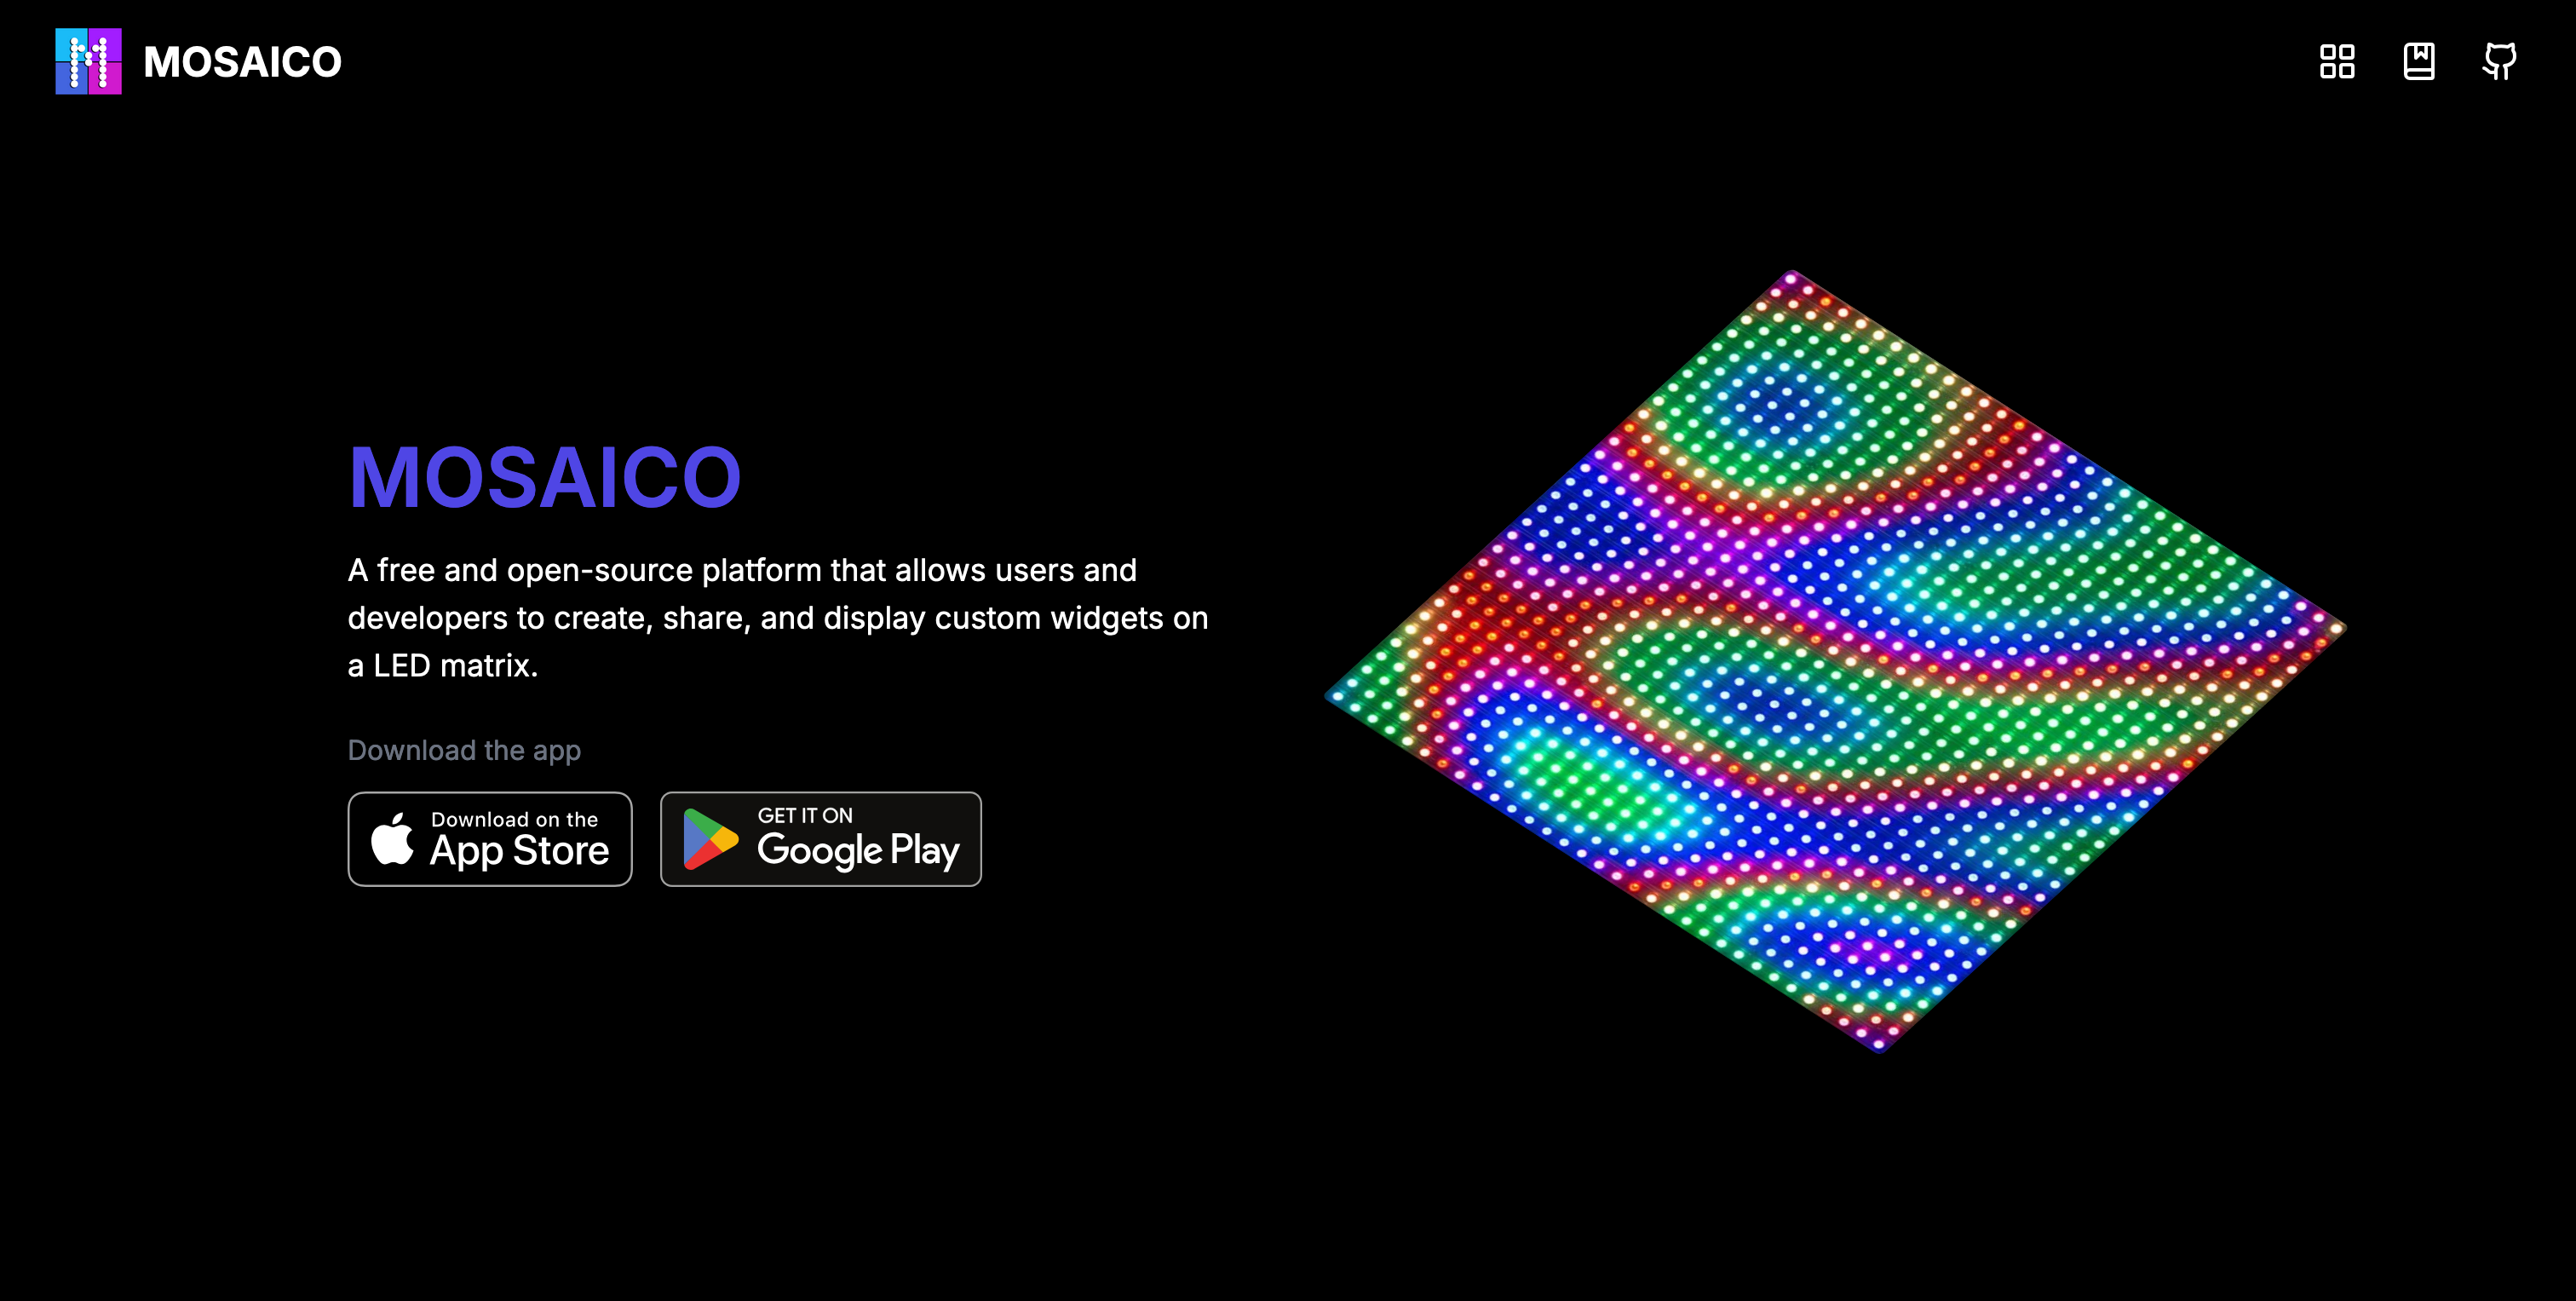
\includegraphics[width=\textwidth]{tesi/img/website_demo/landing/1.png}
\caption*{Call to action}
\end{minipage}
\begin{minipage}[b]{0.49\textwidth}
\centering
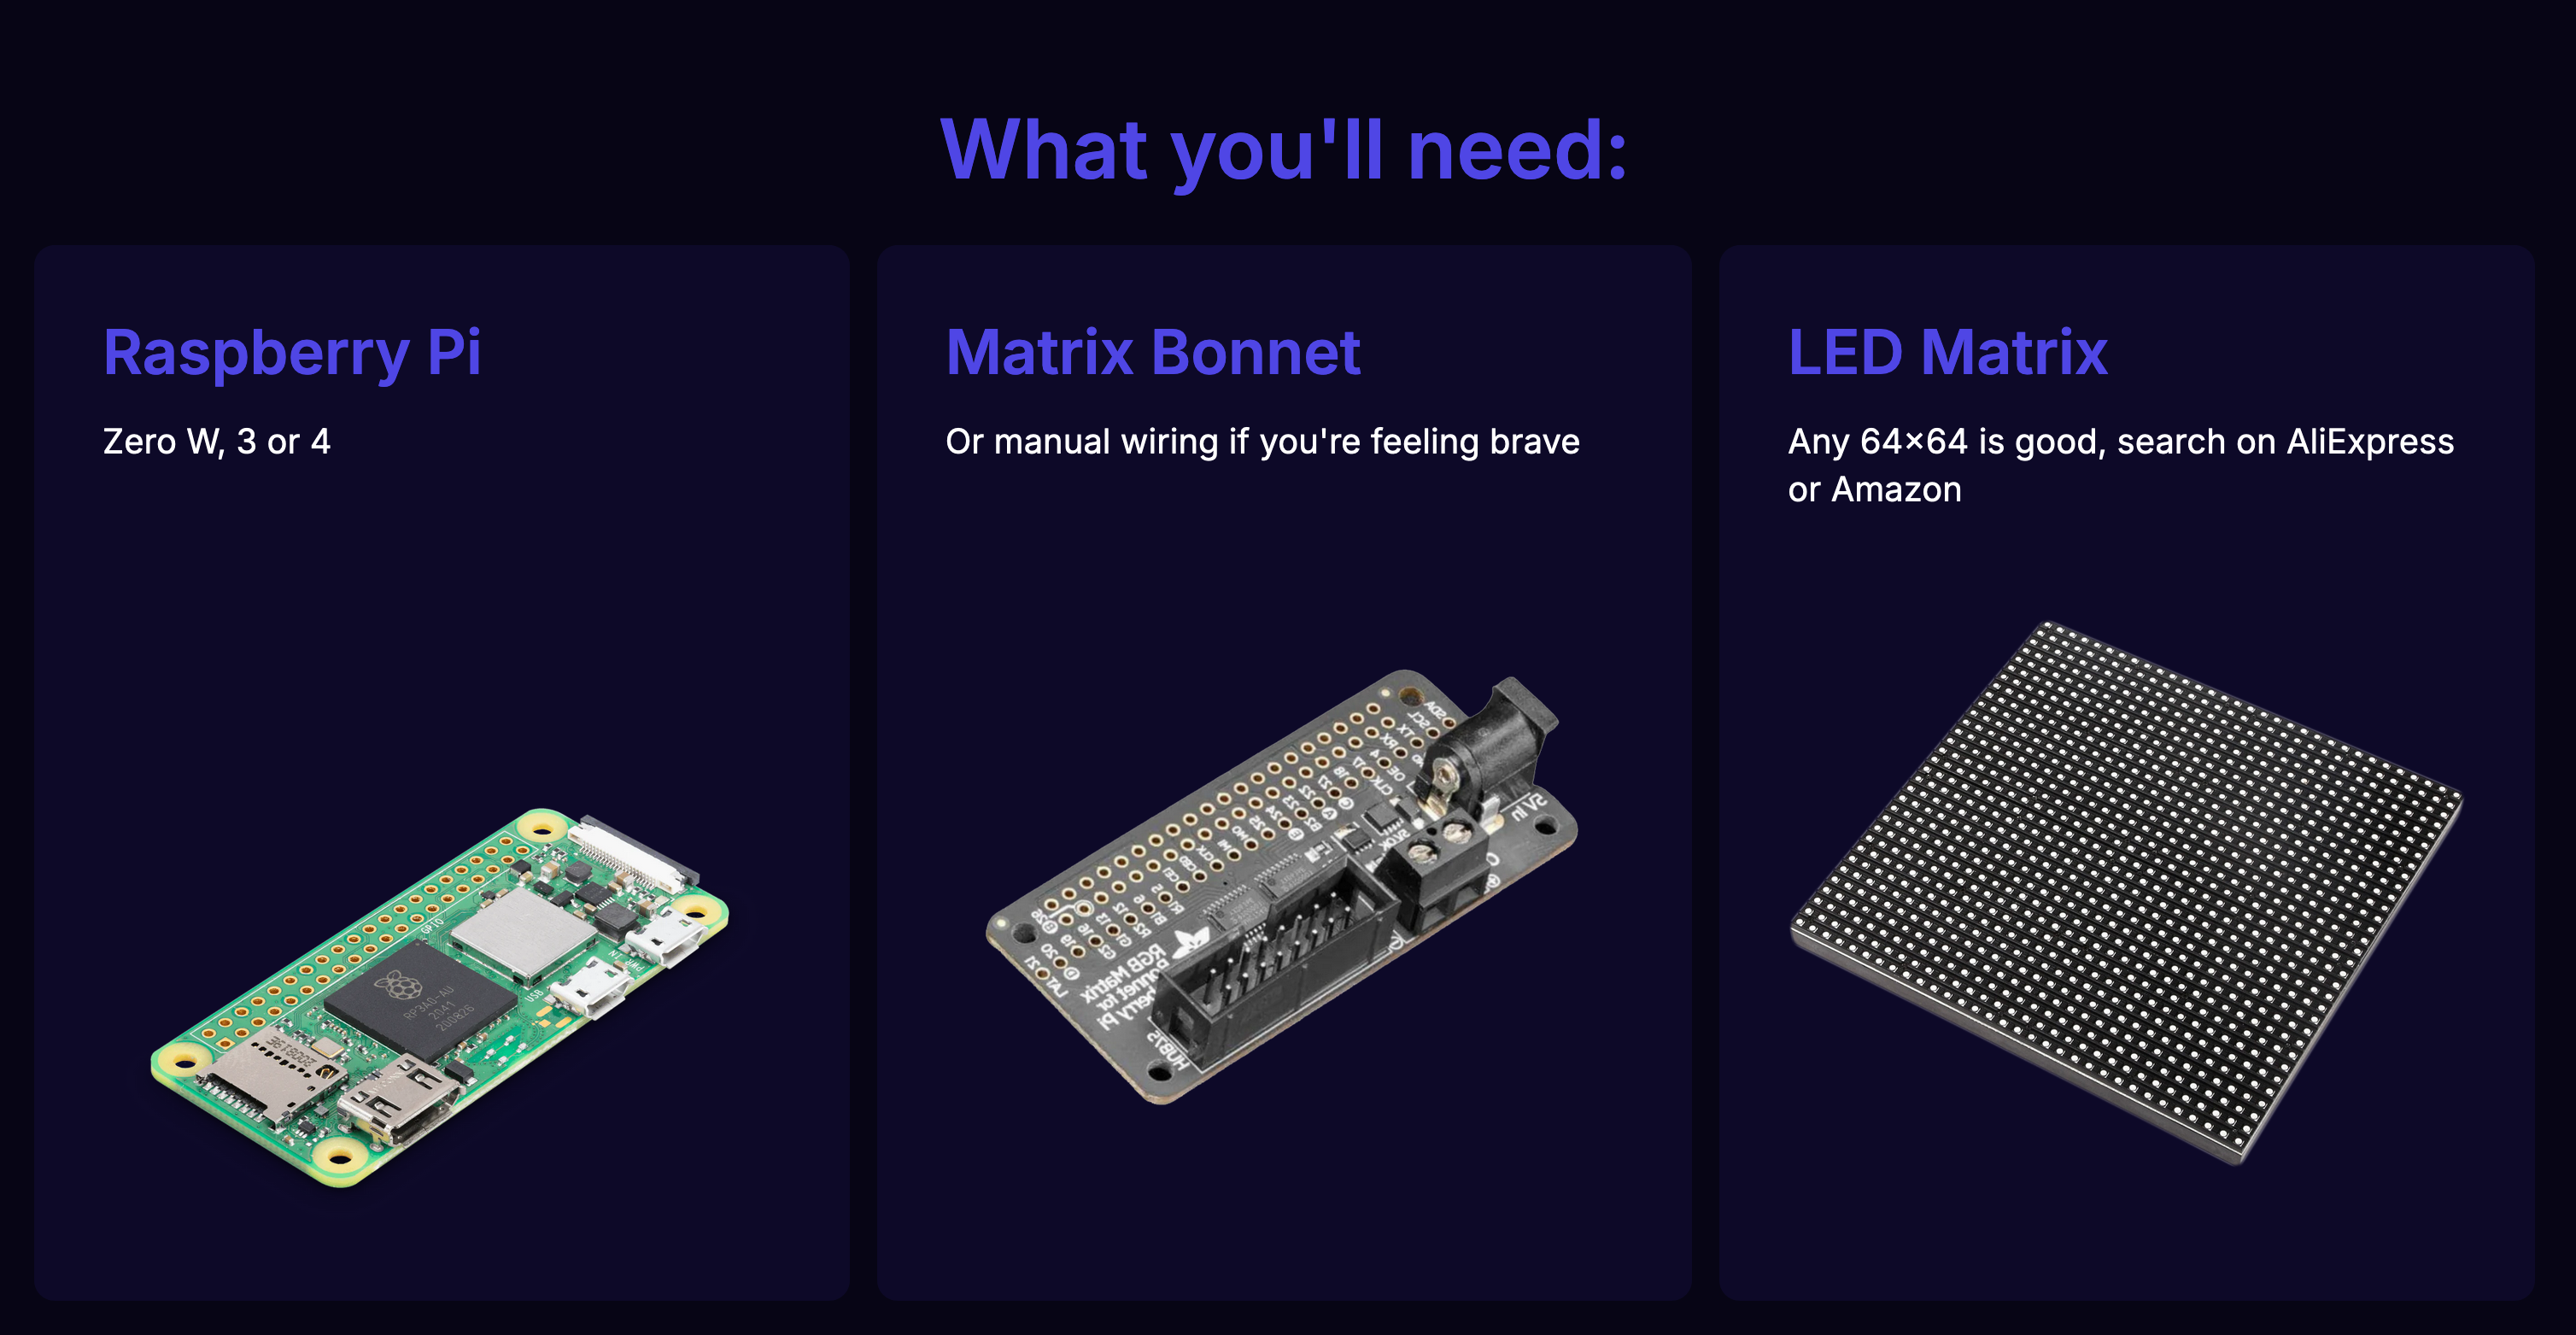
\includegraphics[width=\textwidth]{tesi/img/website_demo/landing/2.png}
\caption*{Hardware components}
\end{minipage}
\end{figure}

\begin{figure}[H]
\centering
\begin{minipage}[b]{0.49\textwidth}
\centering
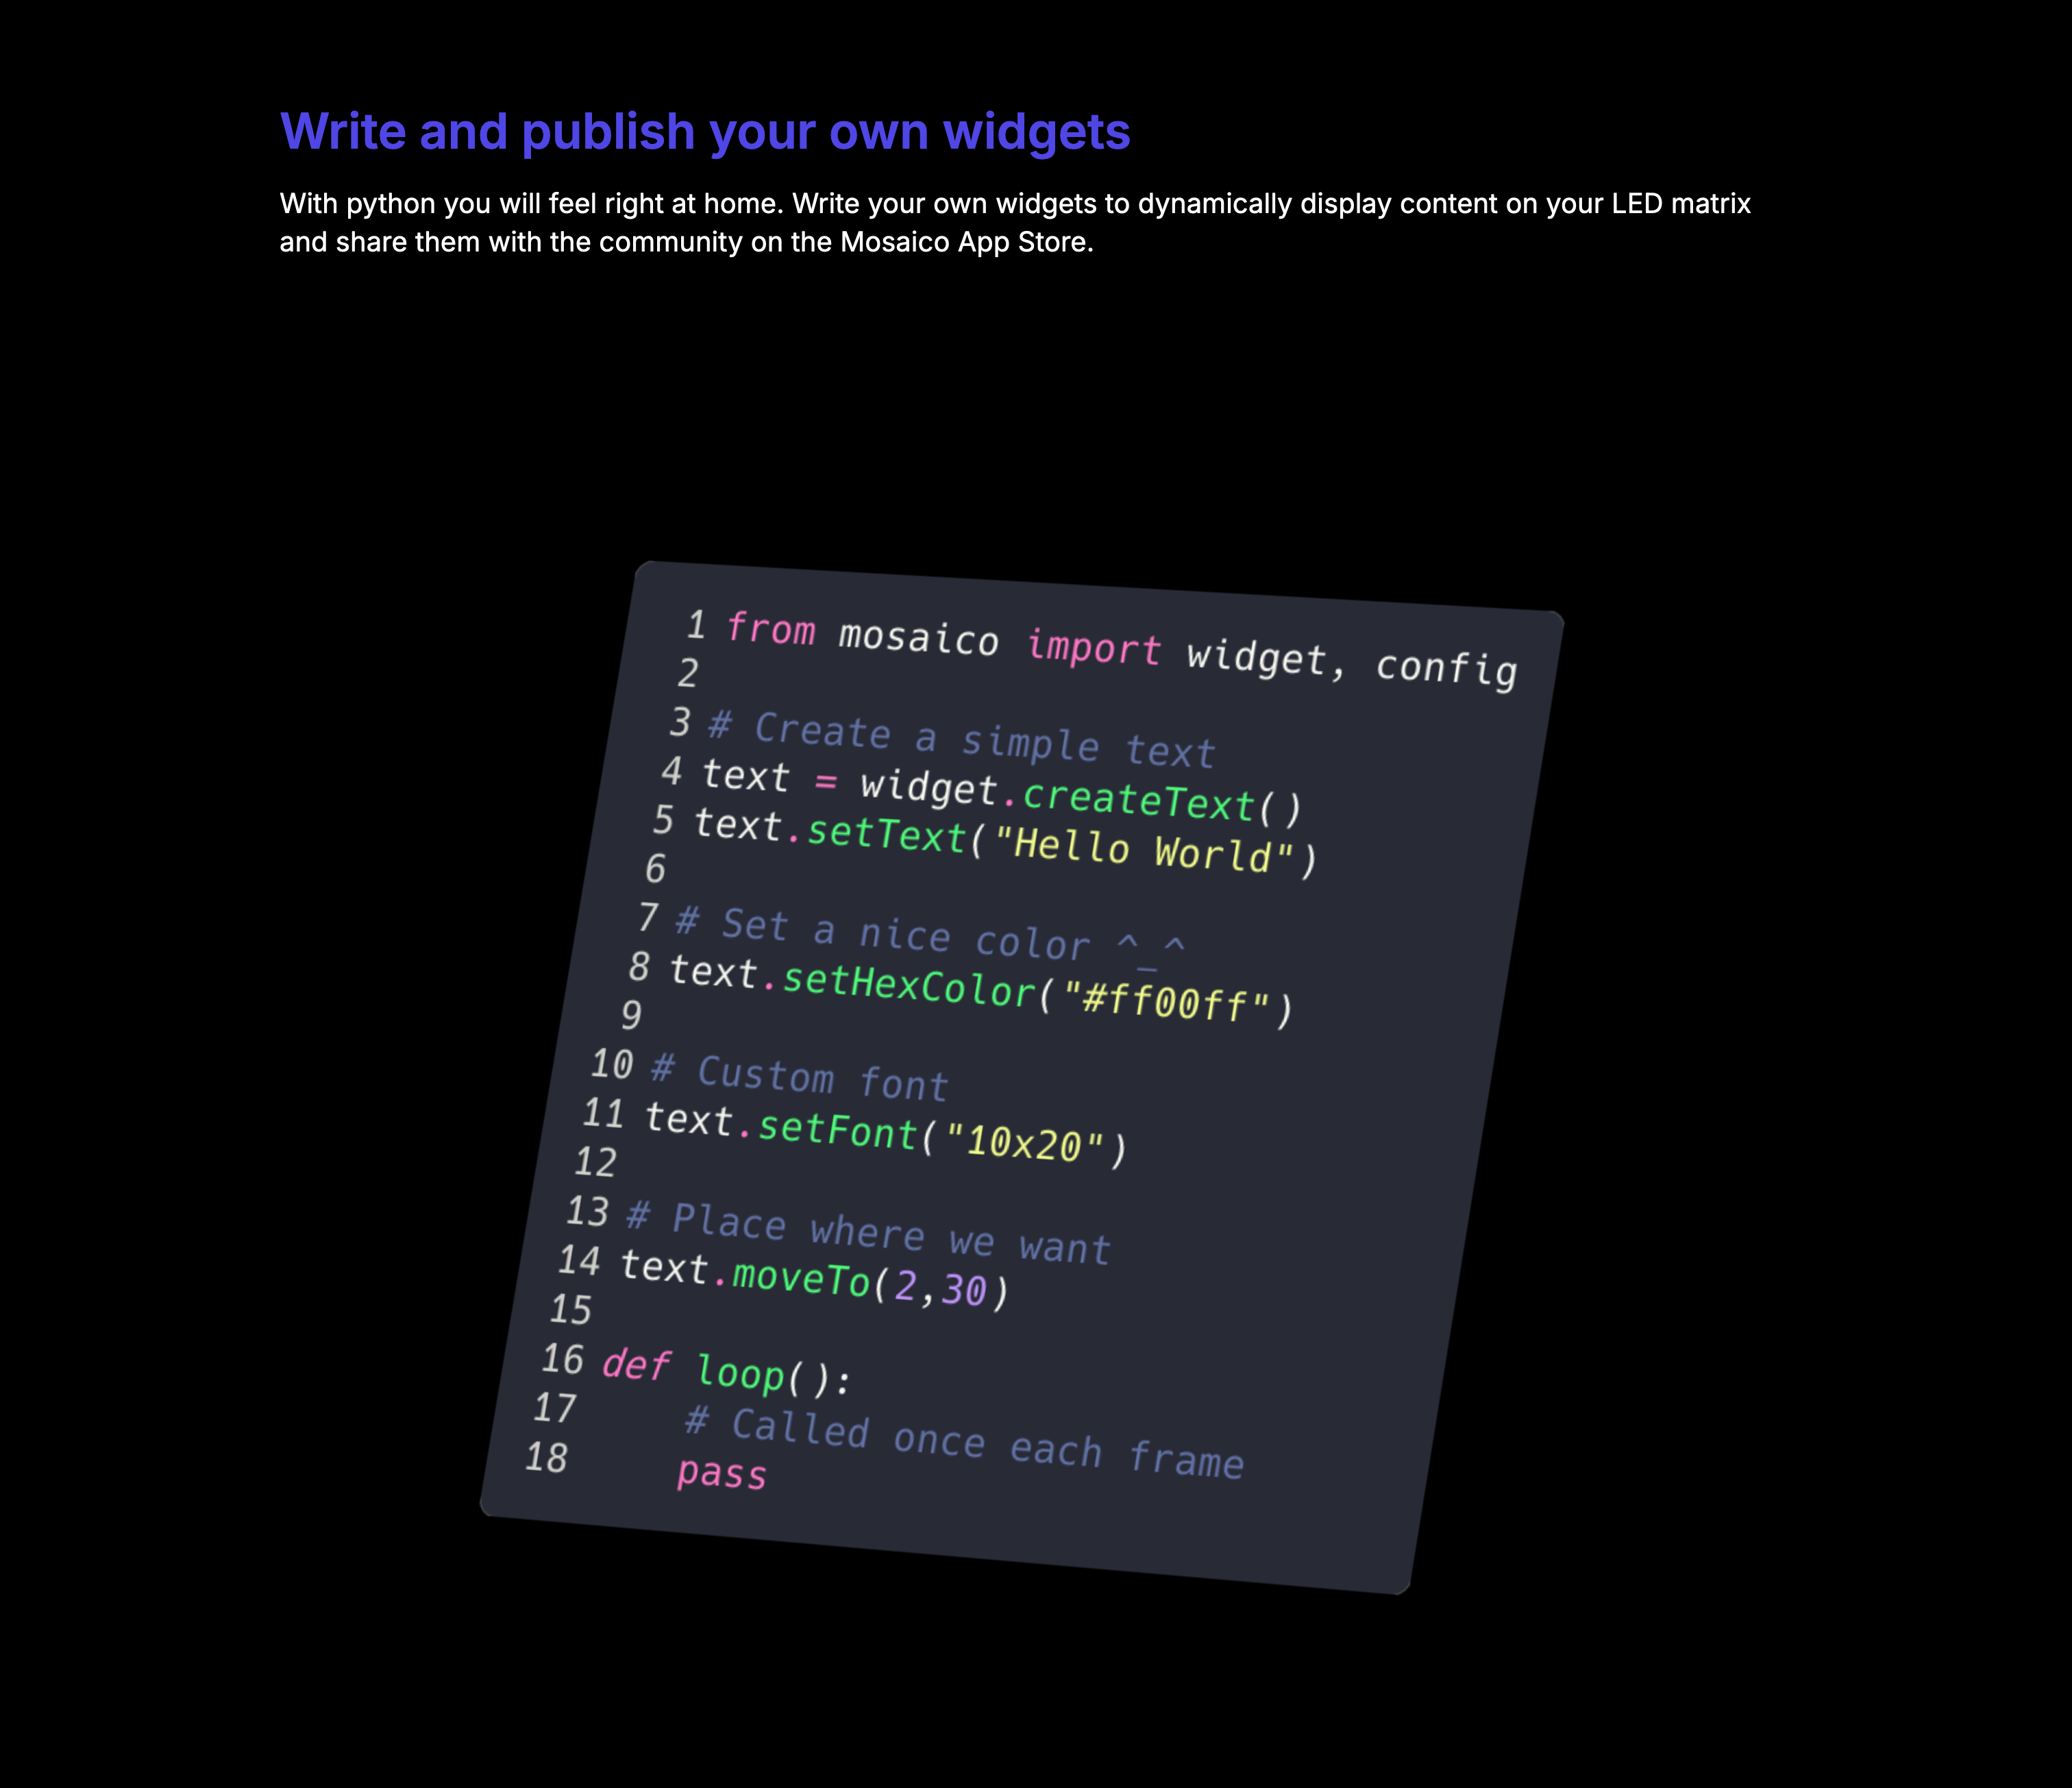
\includegraphics[width=\textwidth]{tesi/img/website_demo/landing/3.png}
\caption*{Widgets}
\end{minipage}
\begin{minipage}[b]{0.49\textwidth}
\centering
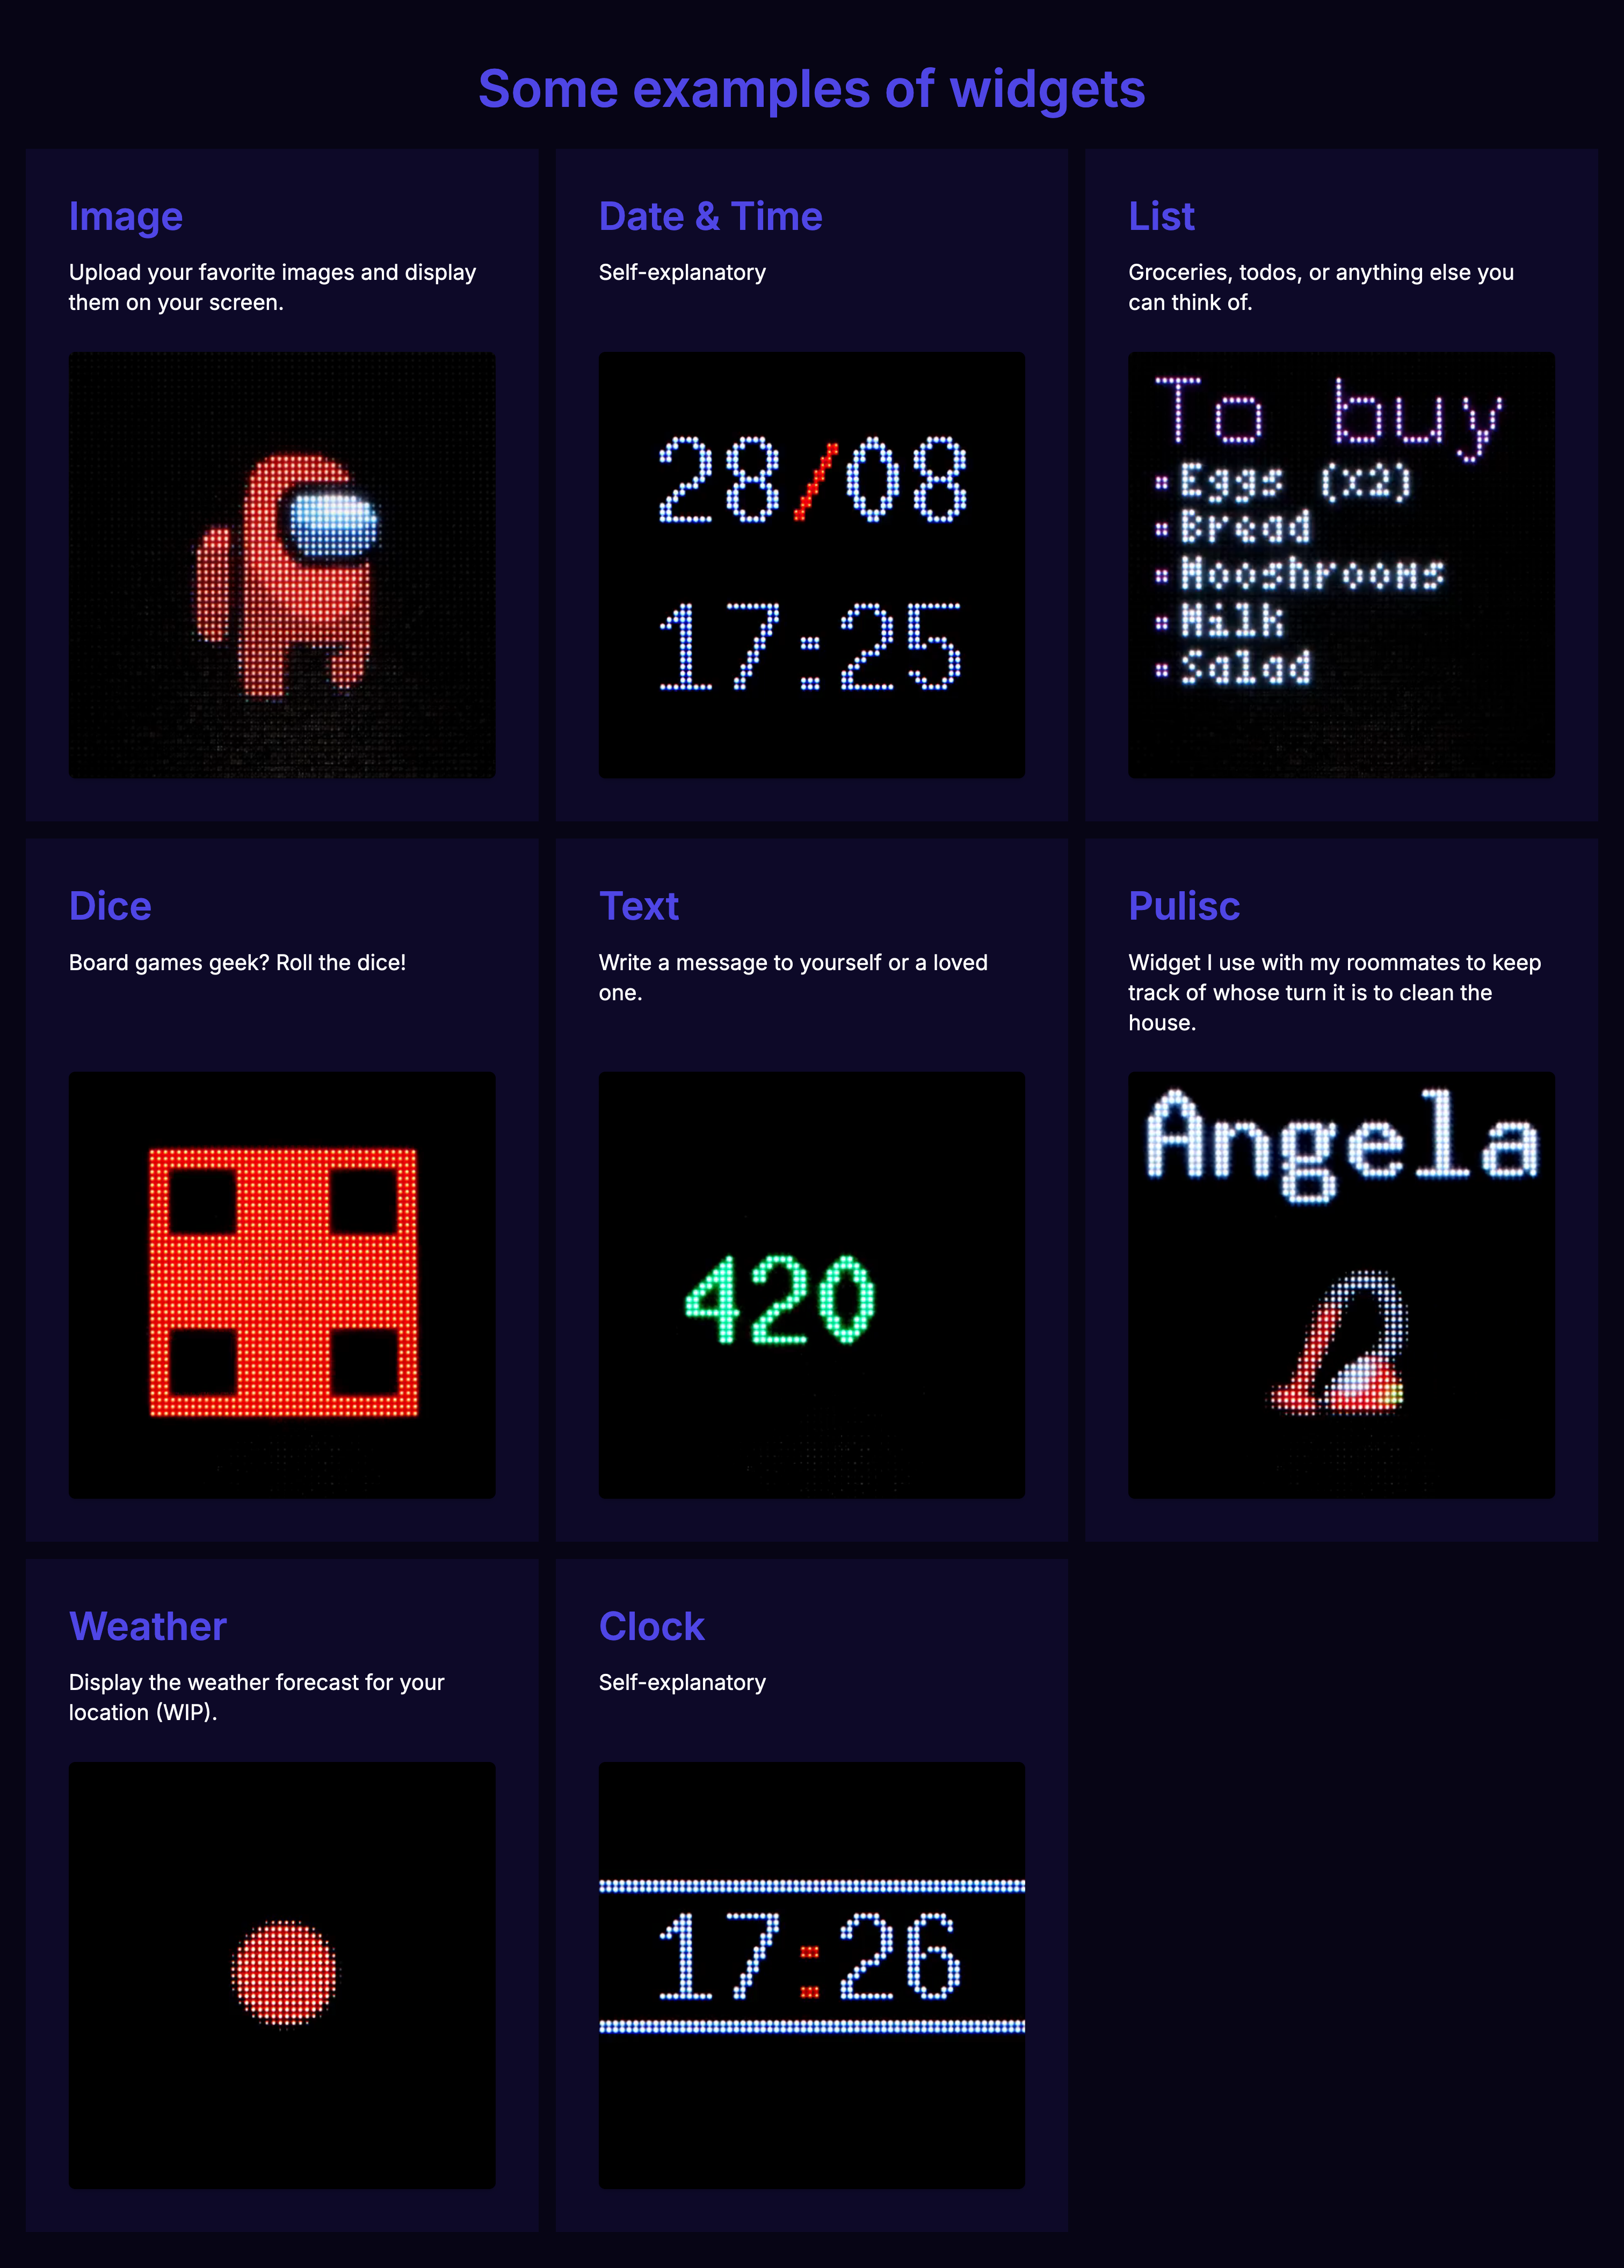
\includegraphics[width=\textwidth]{tesi/img/website_demo/landing/4.png}
\caption*{Widgets showcase}
\end{minipage}
\end{figure}

\begin{figure}[H]
\centering
\begin{minipage}[b]{0.49\textwidth}
\centering
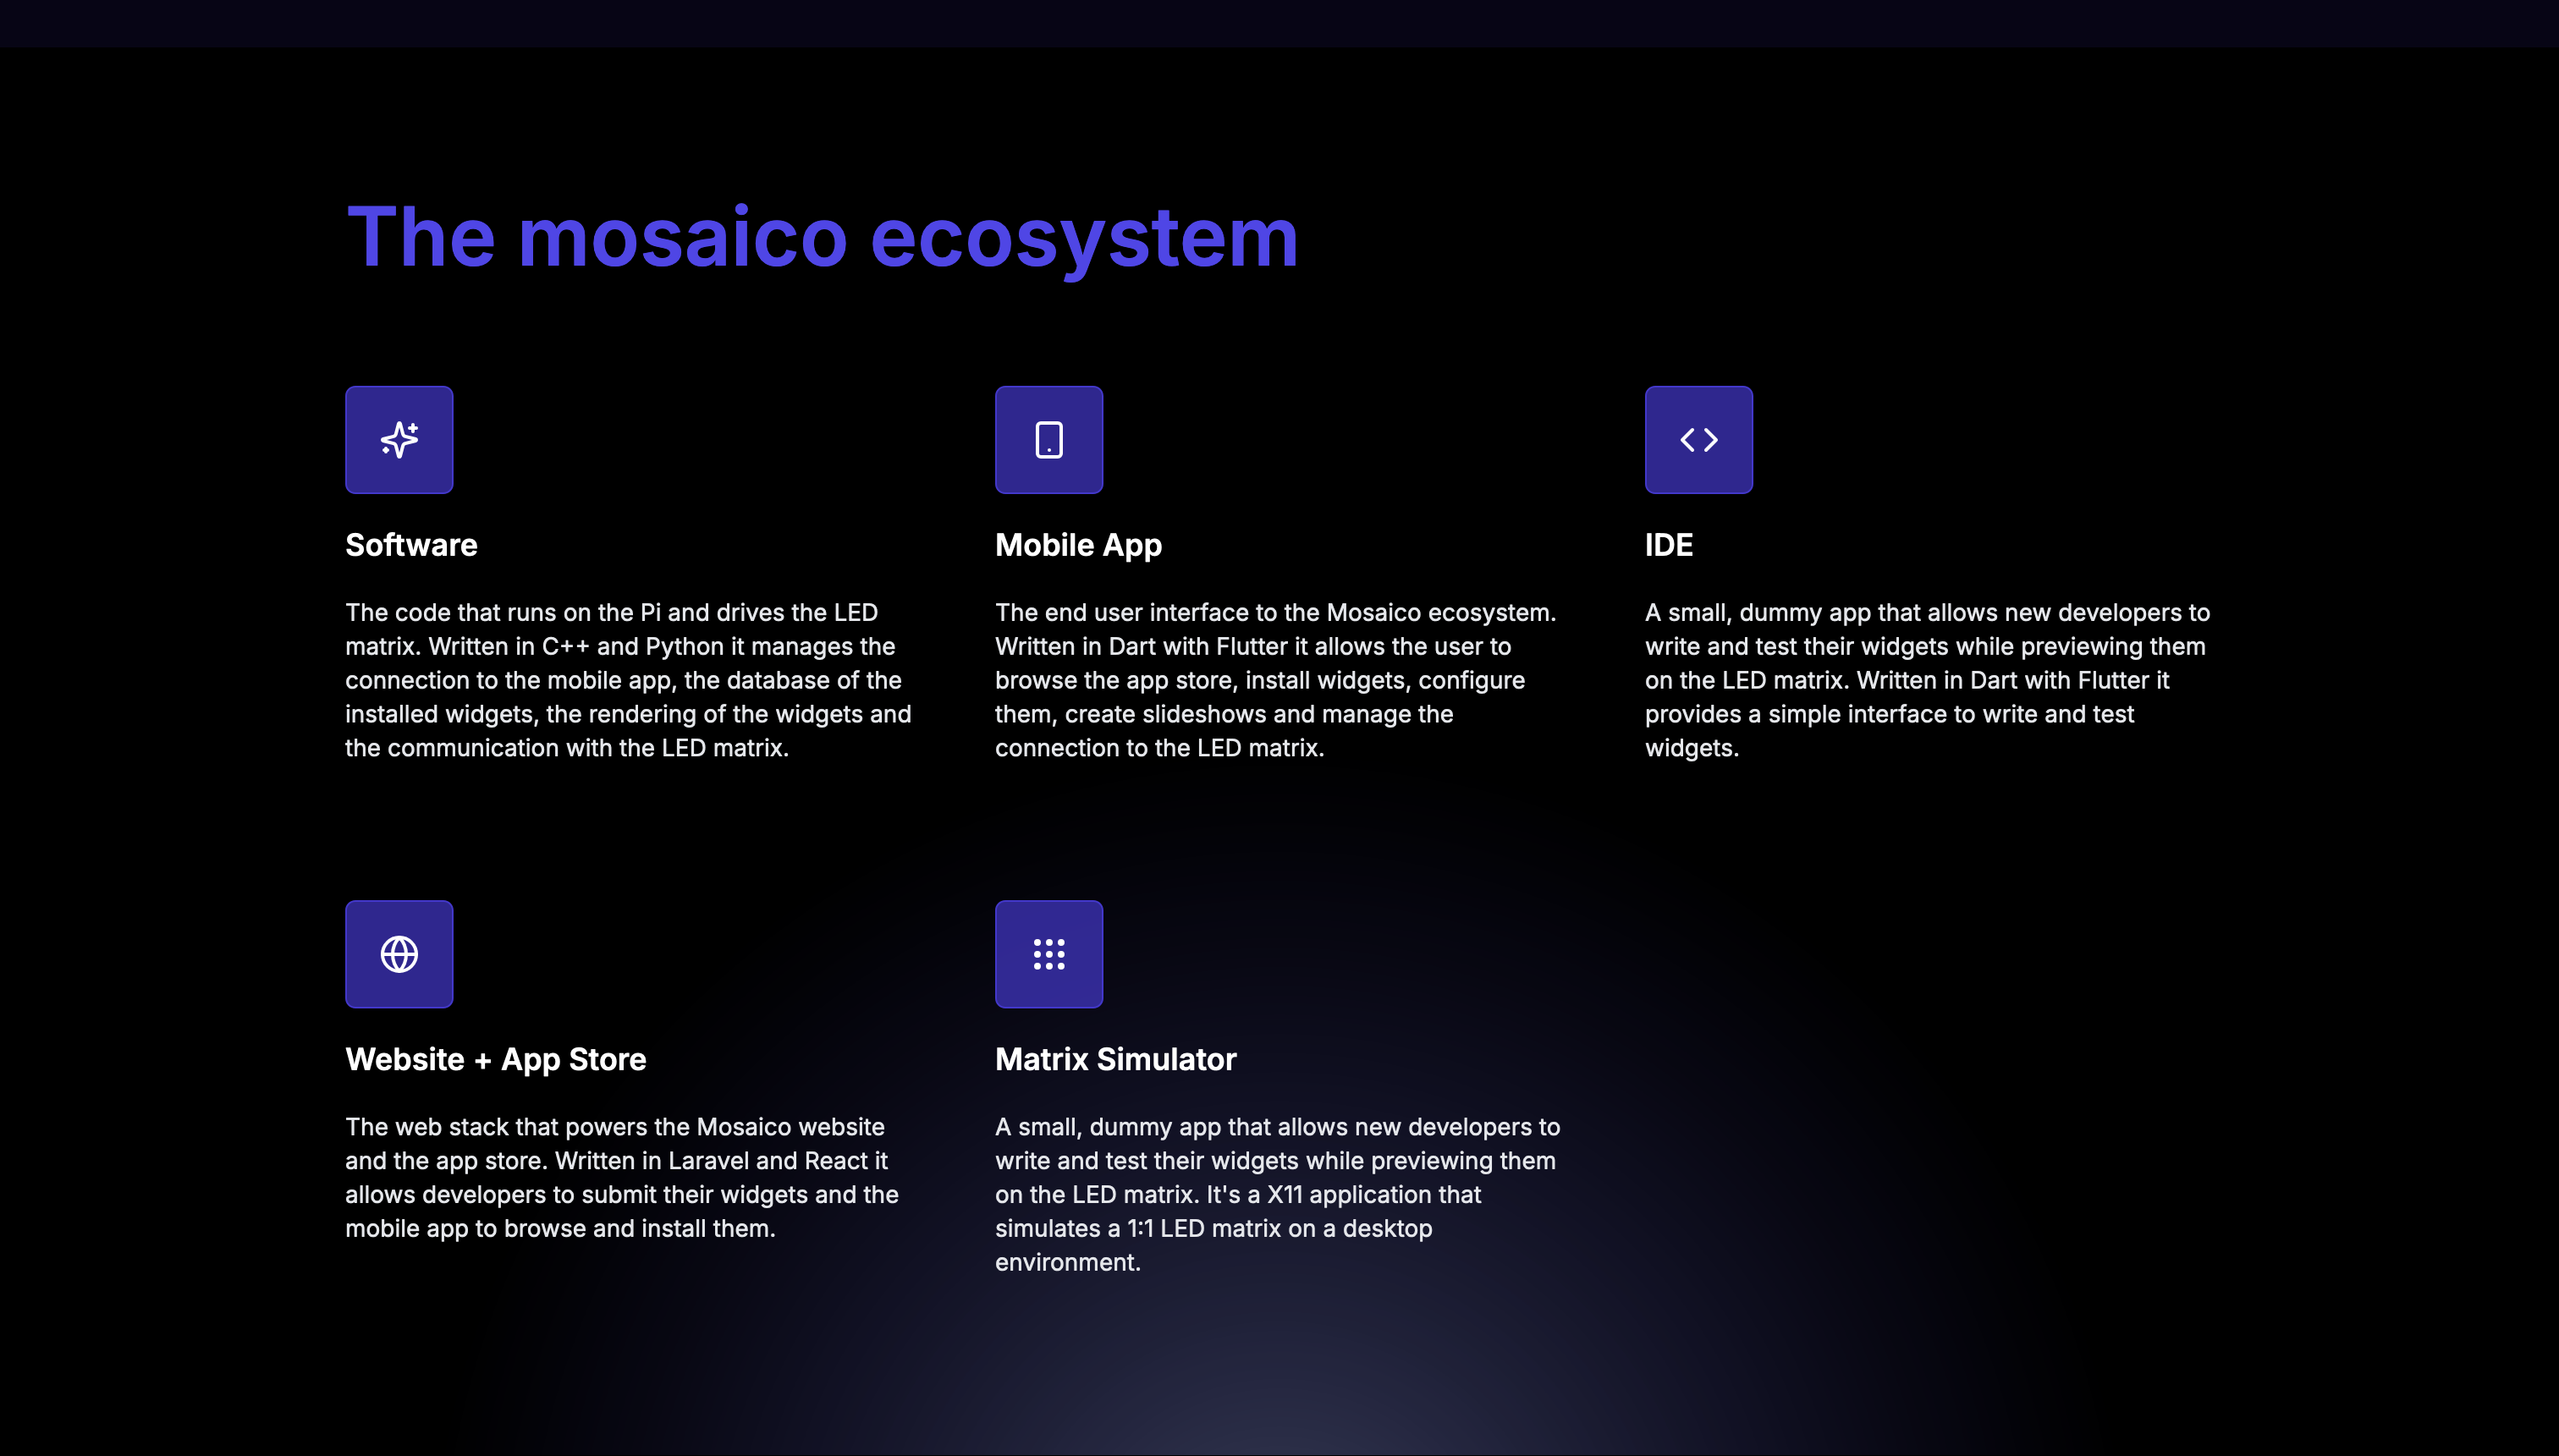
\includegraphics[width=\textwidth]{tesi/img/website_demo/landing/5.png}
\caption*{The ecosystem}
\end{minipage}
\begin{minipage}[b]{0.49\textwidth}
\centering
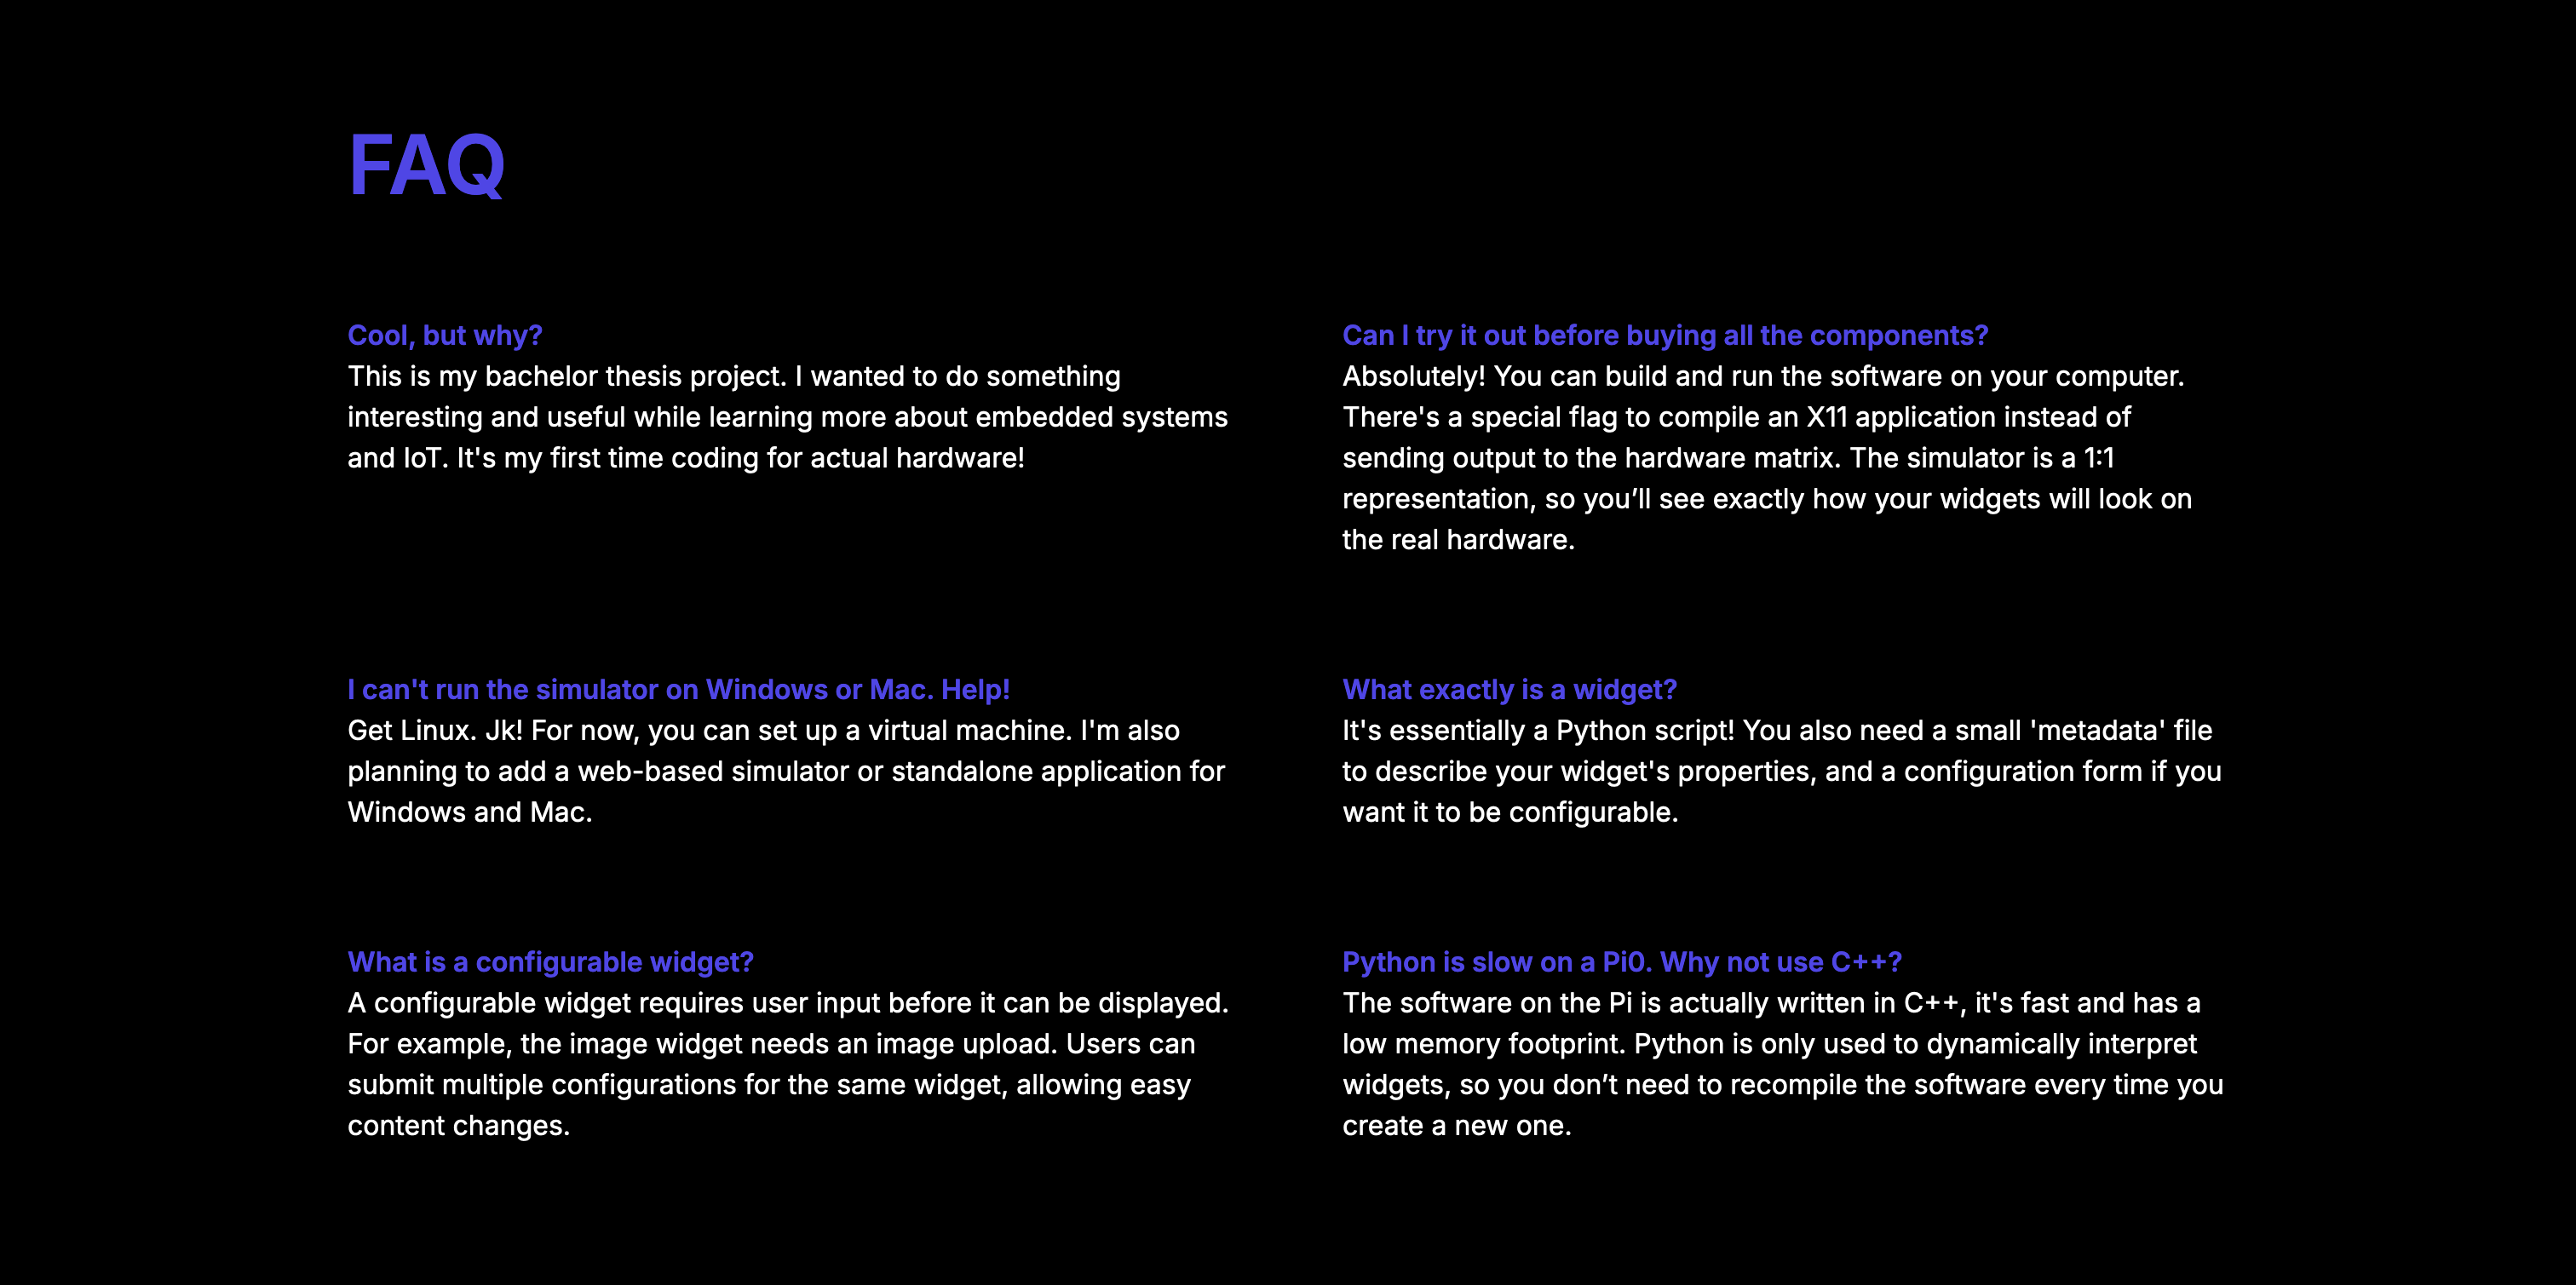
\includegraphics[width=\textwidth]{tesi/img/website_demo/landing/6.png}
\caption*{FAQ}
\end{minipage}
\end{figure}
